
%% bare_adv.tex
%% V1.4b
%% 2015/08/26
%% by Michael Shell
%% See: 
%% http://www.michaelshell.org/
%% for current contact information.
%%
%% This is a skeleton file demonstrating the advanced use of IEEEtran.cls
%% (requires IEEEtran.cls version 1.8b or later) with an IEEE Computer
%% Society journal paper.
%%
%% Support sites:
%% http://www.michaelshell.org/tex/ieeetran/
%% http://www.ctan.org/pkg/ieeetran
%% and
%% http://www.ieee.org/

%%*************************************************************************
%% Legal Notice:
%% This code is offered as-is without any warranty either expressed or
%% implied; without even the implied warranty of MERCHANTABILITY or
%% FITNESS FOR A PARTICULAR PURPOSE! 
%% User assumes all risk.
%% In no event shall the IEEE or any contributor to this code be liable for
%% any damages or losses, including, but not limited to, incidental,
%% consequential, or any other damages, resulting from the use or misuse
%% of any information contained here.
%%
%% All comments are the opinions of their respective authors and are not
%% necessarily endorsed by the IEEE.
%%
%% This work is distributed under the LaTeX Project Public License (LPPL)
%% ( http://www.latex-project.org/ ) version 1.3, and may be freely used,
%% distributed and modified. A copy of the LPPL, version 1.3, is included
%% in the base LaTeX documentation of all distributions of LaTeX released
%% 2003/12/01 or later.
%% Retain all contribution notices and credits.
%% ** Modified files should be clearly indicated as such, including  **
%% ** renaming them and changing author support contact information. **
%%*************************************************************************


% *** Authors should verify (and, if needed, correct) their LaTeX system  ***
% *** with the testflow diagnostic prior to trusting their LaTeX platform ***
% *** with production work. The IEEE's font choices and paper sizes can   ***
% *** trigger bugs that do not appear when using other class files.       ***                          ***
% The testflow support page is at:
% http://www.michaelshell.org/tex/testflow/


% IEEEtran V1.7 and later provides for these CLASSINPUT macros to allow the
% user to reprogram some IEEEtran.cls defaults if needed. These settings
% override the internal defaults of IEEEtran.cls regardless of which class
% options are used. Do not use these unless you have good reason to do so as
% they can result in nonIEEE compliant documents. User beware. ;)
%
%\newcommand{\CLASSINPUTbaselinestretch}{1.0} % baselinestretch
%\newcommand{\CLASSINPUTinnersidemargin}{1in} % inner side margin
%\newcommand{\CLASSINPUToutersidemargin}{1in} % outer side margin
%\newcommand{\CLASSINPUTtoptextmargin}{1in}   % top text margin
%\newcommand{\CLASSINPUTbottomtextmargin}{1in}% bottom text margin




%
\documentclass[10pt,journal,compsoc]{IEEEtran}
% If IEEEtran.cls has not been installed into the LaTeX system files,
% manually specify the path to it like:
% \documentclass[10pt,journal,compsoc]{../sty/IEEEtran}


% For Computer Society journals, IEEEtran defaults to the use of 
% Palatino/Palladio as is done in IEEE Computer Society journals.
% To go back to Times Roman, you can use this code:
%\renewcommand{\rmdefault}{ptm}\selectfont





% Some very useful LaTeX packages include:
% (uncomment the ones you want to load)



% *** MISC UTILITY PACKAGES ***
%
%\usepackage{ifpdf}
% Heiko Oberdiek's ifpdf.sty is very useful if you need conditional
% compilation based on whether the output is pdf or dvi.
% usage:
% \ifpdf
%   % pdf code
% \else
%   % dvi code
% \fi
% The latest version of ifpdf.sty can be obtained from:
% http://www.ctan.org/pkg/ifpdf
% Also, note that IEEEtran.cls V1.7 and later provides a builtin
% \ifCLASSINFOpdf conditional that works the same way.
% When switching from latex to pdflatex and vice-versa, the compiler may
% have to be run twice to clear warning/error messages.






% *** CITATION PACKAGES ***
%
\ifCLASSOPTIONcompsoc
  % The IEEE Computer Society needs nocompress option
  % requires cite.sty v4.0 or later (November 2003)
  \usepackage[nocompress]{cite}
\else
  % normal IEEE
  \usepackage{cite}
\fi
% cite.sty was written by Donald Arseneau
% V1.6 and later of IEEEtran pre-defines the format of the cite.sty package
% \cite{} output to follow that of the IEEE. Loading the cite package will
% result in citation numbers being automatically sorted and properly
% "compressed/ranged". e.g., [1], [9], [2], [7], [5], [6] without using
% cite.sty will become [1], [2], [5]--[7], [9] using cite.sty. cite.sty's
% \cite will automatically add leading space, if needed. Use cite.sty's
% noadjust option (cite.sty V3.8 and later) if you want to turn this off
% such as if a citation ever needs to be enclosed in parenthesis.
% cite.sty is already installed on most LaTeX systems. Be sure and use
% version 5.0 (2009-03-20) and later if using hyperref.sty.
% The latest version can be obtained at:
% http://www.ctan.org/pkg/cite
% The documentation is contained in the cite.sty file itself.
%
% Note that some packages require special options to format as the Computer
% Society requires. In particular, Computer Society  papers do not use
% compressed citation ranges as is done in typical IEEE papers
% (e.g., [1]-[4]). Instead, they list every citation separately in order
% (e.g., [1], [2], [3], [4]). To get the latter we need to load the cite
% package with the nocompress option which is supported by cite.sty v4.0
% and later.





% *** GRAPHICS RELATED PACKAGES ***
%
\ifCLASSINFOpdf
  % \usepackage[pdftex]{graphicx}
  % declare the path(s) where your graphic files are
  % \graphicspath{{../pdf/}{../jpeg/}}
  % and their extensions so you won't have to specify these with
  % every instance of \includegraphics
  % \DeclareGraphicsExtensions{.pdf,.jpeg,.png}
\else
  % or other class option (dvipsone, dvipdf, if not using dvips). graphicx
  % will default to the driver specified in the system graphics.cfg if no
  % driver is specified.
  % \usepackage[dvips]{graphicx}
  % declare the path(s) where your graphic files are
  % \graphicspath{{../eps/}}
  % and their extensions so you won't have to specify these with
  % every instance of \includegraphics
  % \DeclareGraphicsExtensions{.eps}
\fi
% graphicx was written by David Carlisle and Sebastian Rahtz. It is
% required if you want graphics, photos, etc. graphicx.sty is already
% installed on most LaTeX systems. The latest version and documentation
% can be obtained at: 
% http://www.ctan.org/pkg/graphicx
% Another good source of documentation is "Using Imported Graphics in
% LaTeX2e" by Keith Reckdahl which can be found at:
% http://www.ctan.org/pkg/epslatex
%
% latex, and pdflatex in dvi mode, support graphics in encapsulated
% postscript (.eps) format. pdflatex in pdf mode supports graphics
% in .pdf, .jpeg, .png and .mps (metapost) formats. Users should ensure
% that all non-photo figures use a vector format (.eps, .pdf, .mps) and
% not a bitmapped formats (.jpeg, .png). The IEEE frowns on bitmapped formats
% which can result in "jaggedy"/blurry rendering of lines and letters as
% well as large increases in file sizes.
%
% You can find documentation about the pdfTeX application at:
% http://www.tug.org/applications/pdftex


%%%%%%%%%%%%%%%%%% MY OWN IMPORTED PACKAGES!!!!! %%%%%%%%%%%%%%%%%%
\usepackage{graphicx}
\graphicspath{{Images/}}
\usepackage{minted}
\usepackage{multicol}
\usepackage{hyperref}

% *** MATH PACKAGES ***
%
%\usepackage{amsmath}
% A popular package from the American Mathematical Society that provides
% many useful and powerful commands for dealing with mathematics.
%
% Note that the amsmath package sets \interdisplaylinepenalty to 10000
% thus preventing page breaks from occurring within multiline equations. Use:
%\interdisplaylinepenalty=2500
% after loading amsmath to restore such page breaks as IEEEtran.cls normally
% does. amsmath.sty is already installed on most LaTeX systems. The latest
% version and documentation can be obtained at:
% http://www.ctan.org/pkg/amsmath





% *** SPECIALIZED LIST PACKAGES ***
%\usepackage{acronym}
% acronym.sty was written by Tobias Oetiker. This package provides tools for
% managing documents with large numbers of acronyms. (You don't *have* to
% use this package - unless you have a lot of acronyms, you may feel that
% such package management of them is bit of an overkill.)
% Do note that the acronym environment (which lists acronyms) will have a
% problem when used under IEEEtran.cls because acronym.sty relies on the
% description list environment - which IEEEtran.cls has customized for
% producing IEEE style lists. A workaround is to declared the longest
% label width via the IEEEtran.cls \IEEEiedlistdecl global control:
%
% \renewcommand{\IEEEiedlistdecl}{\IEEEsetlabelwidth{SONET}}
% \begin{acronym}
%
% \end{acronym}
% \renewcommand{\IEEEiedlistdecl}{\relax}% remember to reset \IEEEiedlistdecl
%
% instead of using the acronym environment's optional argument.
% The latest version and documentation can be obtained at:
% http://www.ctan.org/pkg/acronym


%\usepackage{algorithmic}
% algorithmic.sty was written by Peter Williams and Rogerio Brito.
% This package provides an algorithmic environment fo describing algorithms.
% You can use the algorithmic environment in-text or within a figure
% environment to provide for a floating algorithm. Do NOT use the algorithm
% floating environment provided by algorithm.sty (by the same authors) or
% algorithm2e.sty (by Christophe Fiorio) as the IEEE does not use dedicated
% algorithm float types and packages that provide these will not provide
% correct IEEE style captions. The latest version and documentation of
% algorithmic.sty can be obtained at:
% http://www.ctan.org/pkg/algorithms
% Also of interest may be the (relatively newer and more customizable)
% algorithmicx.sty package by Szasz Janos:
% http://www.ctan.org/pkg/algorithmicx




% *** ALIGNMENT PACKAGES ***
%
%\usepackage{array}
% Frank Mittelbach's and David Carlisle's array.sty patches and improves
% the standard LaTeX2e array and tabular environments to provide better
% appearance and additional user controls. As the default LaTeX2e table
% generation code is lacking to the point of almost being broken with
% respect to the quality of the end results, all users are strongly
% advised to use an enhanced (at the very least that provided by array.sty)
% set of table tools. array.sty is already installed on most systems. The
% latest version and documentation can be obtained at:
% http://www.ctan.org/pkg/array


%\usepackage{mdwmath}
%\usepackage{mdwtab}
% Also highly recommended is Mark Wooding's extremely powerful MDW tools,
% especially mdwmath.sty and mdwtab.sty which are used to format equations
% and tables, respectively. The MDWtools set is already installed on most
% LaTeX systems. The lastest version and documentation is available at:
% http://www.ctan.org/pkg/mdwtools


% IEEEtran contains the IEEEeqnarray family of commands that can be used to
% generate multiline equations as well as matrices, tables, etc., of high
% quality.


%\usepackage{eqparbox}
% Also of notable interest is Scott Pakin's eqparbox package for creating
% (automatically sized) equal width boxes - aka "natural width parboxes".
% Available at:
% http://www.ctan.org/pkg/eqparbox




% *** SUBFIGURE PACKAGES ***
%\ifCLASSOPTIONcompsoc
%  \usepackage[caption=false,font=footnotesize,labelfont=sf,textfont=sf]{subfig}
%\else
%  \usepackage[caption=false,font=footnotesize]{subfig}
%\fi
% subfig.sty, written by Steven Douglas Cochran, is the modern replacement
% for subfigure.sty, the latter of which is no longer maintained and is
% incompatible with some LaTeX packages including fixltx2e. However,
% subfig.sty requires and automatically loads Axel Sommerfeldt's caption.sty
% which will override IEEEtran.cls' handling of captions and this will result
% in non-IEEE style figure/table captions. To prevent this problem, be sure
% and invoke subfig.sty's "caption=false" package option (available since
% subfig.sty version 1.3, 2005/06/28) as this is will preserve IEEEtran.cls
% handling of captions.
% Note that the Computer Society format requires a sans serif font rather
% than the serif font used in traditional IEEE formatting and thus the need
% to invoke different subfig.sty package options depending on whether
% compsoc mode has been enabled.
%
% The latest version and documentation of subfig.sty can be obtained at:
% http://www.ctan.org/pkg/subfig




% *** FLOAT PACKAGES ***
%
%\usepackage{fixltx2e}
% fixltx2e, the successor to the earlier fix2col.sty, was written by
% Frank Mittelbach and David Carlisle. This package corrects a few problems
% in the LaTeX2e kernel, the most notable of which is that in current
% LaTeX2e releases, the ordering of single and double column floats is not
% guaranteed to be preserved. Thus, an unpatched LaTeX2e can allow a
% single column figure to be placed prior to an earlier double column
% figure.
% Be aware that LaTeX2e kernels dated 2015 and later have fixltx2e.sty's
% corrections already built into the system in which case a warning will
% be issued if an attempt is made to load fixltx2e.sty as it is no longer
% needed.
% The latest version and documentation can be found at:
% http://www.ctan.org/pkg/fixltx2e


%\usepackage{stfloats}
% stfloats.sty was written by Sigitas Tolusis. This package gives LaTeX2e
% the ability to do double column floats at the bottom of the page as well
% as the top. (e.g., "\begin{figure*}[!b]" is not normally possible in
% LaTeX2e). It also provides a command:
%\fnbelowfloat
% to enable the placement of footnotes below bottom floats (the standard
% LaTeX2e kernel puts them above bottom floats). This is an invasive package
% which rewrites many portions of the LaTeX2e float routines. It may not work
% with other packages that modify the LaTeX2e float routines. The latest
% version and documentation can be obtained at:
% http://www.ctan.org/pkg/stfloats
% Do not use the stfloats baselinefloat ability as the IEEE does not allow
% \baselineskip to stretch. Authors submitting work to the IEEE should note
% that the IEEE rarely uses double column equations and that authors should try
% to avoid such use. Do not be tempted to use the cuted.sty or midfloat.sty
% packages (also by Sigitas Tolusis) as the IEEE does not format its papers in
% such ways.
% Do not attempt to use stfloats with fixltx2e as they are incompatible.
% Instead, use Morten Hogholm'a dblfloatfix which combines the features
% of both fixltx2e and stfloats:
%
% \usepackage{dblfloatfix}
% The latest version can be found at:
% http://www.ctan.org/pkg/dblfloatfix


%\ifCLASSOPTIONcaptionsoff
%  \usepackage[nomarkers]{endfloat}
% \let\MYoriglatexcaption\caption
% \renewcommand{\caption}[2][\relax]{\MYoriglatexcaption[#2]{#2}}
%\fi
% endfloat.sty was written by James Darrell McCauley, Jeff Goldberg and 
% Axel Sommerfeldt. This package may be useful when used in conjunction with 
% IEEEtran.cls'  captionsoff option. Some IEEE journals/societies require that
% submissions have lists of figures/tables at the end of the paper and that
% figures/tables without any captions are placed on a page by themselves at
% the end of the document. If needed, the draftcls IEEEtran class option or
% \CLASSINPUTbaselinestretch interface can be used to increase the line
% spacing as well. Be sure and use the nomarkers option of endfloat to
% prevent endfloat from "marking" where the figures would have been placed
% in the text. The two hack lines of code above are a slight modification of
% that suggested by in the endfloat docs (section 8.4.1) to ensure that
% the full captions always appear in the list of figures/tables - even if
% the user used the short optional argument of \caption[]{}.
% IEEE papers do not typically make use of \caption[]'s optional argument,
% so this should not be an issue. A similar trick can be used to disable
% captions of packages such as subfig.sty that lack options to turn off
% the subcaptions:
% For subfig.sty:
% \let\MYorigsubfloat\subfloat
% \renewcommand{\subfloat}[2][\relax]{\MYorigsubfloat[]{#2}}
% However, the above trick will not work if both optional arguments of
% the \subfloat command are used. Furthermore, there needs to be a
% description of each subfigure *somewhere* and endfloat does not add
% subfigure captions to its list of figures. Thus, the best approach is to
% avoid the use of subfigure captions (many IEEE journals avoid them anyway)
% and instead reference/explain all the subfigures within the main caption.
% The latest version of endfloat.sty and its documentation can obtained at:
% http://www.ctan.org/pkg/endfloat
%
% The IEEEtran \ifCLASSOPTIONcaptionsoff conditional can also be used
% later in the document, say, to conditionally put the References on a 
% page by themselves.





% *** PDF, URL AND HYPERLINK PACKAGES ***
%
%\usepackage{url}
% url.sty was written by Donald Arseneau. It provides better support for
% handling and breaking URLs. url.sty is already installed on most LaTeX
% systems. The latest version and documentation can be obtained at:
% http://www.ctan.org/pkg/url
% Basically, \url{my_url_here}.


% NOTE: PDF thumbnail features are not required in IEEE papers
%       and their use requires extra complexity and work.
%\ifCLASSINFOpdf
%  \usepackage[pdftex]{thumbpdf}
%\else
%  \usepackage[dvips]{thumbpdf}
%\fi
% thumbpdf.sty and its companion Perl utility were written by Heiko Oberdiek.
% It allows the user a way to produce PDF documents that contain fancy
% thumbnail images of each of the pages (which tools like acrobat reader can
% utilize). This is possible even when using dvi->ps->pdf workflow if the
% correct thumbpdf driver options are used. thumbpdf.sty incorporates the
% file containing the PDF thumbnail information (filename.tpm is used with
% dvips, filename.tpt is used with pdftex, where filename is the base name of
% your tex document) into the final ps or pdf output document. An external
% utility, the thumbpdf *Perl script* is needed to make these .tpm or .tpt
% thumbnail files from a .ps or .pdf version of the document (which obviously
% does not yet contain pdf thumbnails). Thus, one does a:
% 
% thumbpdf filename.pdf 
%
% to make a filename.tpt, and:
%
% thumbpdf --mode dvips filename.ps
%
% to make a filename.tpm which will then be loaded into the document by
% thumbpdf.sty the NEXT time the document is compiled (by pdflatex or
% latex->dvips->ps2pdf). Users must be careful to regenerate the .tpt and/or
% .tpm files if the main document changes and then to recompile the
% document to incorporate the revised thumbnails to ensure that thumbnails
% match the actual pages. It is easy to forget to do this!
% 
% Unix systems come with a Perl interpreter. However, MS Windows users
% will usually have to install a Perl interpreter so that the thumbpdf
% script can be run. The Ghostscript PS/PDF interpreter is also required.
% See the thumbpdf docs for details. The latest version and documentation
% can be obtained at.
% http://www.ctan.org/pkg/thumbpdf


% NOTE: PDF hyperlink and bookmark features are not required in IEEE
%       papers and their use requires extra complexity and work.
% *** IF USING HYPERREF BE SURE AND CHANGE THE EXAMPLE PDF ***
% *** TITLE/SUBJECT/AUTHOR/KEYWORDS INFO BELOW!!           ***
\newcommand\MYhyperrefoptions{bookmarks=true,bookmarksnumbered=true,
pdfpagemode={UseOutlines},plainpages=false,pdfpagelabels=true,
colorlinks=true,linkcolor={black},citecolor={black},urlcolor={black},
pdftitle={Bare Demo of IEEEtran.cls for Computer Society Journals},%<!CHANGE!
pdfsubject={Typesetting},%<!CHANGE!
pdfauthor={Michael D. Shell},%<!CHANGE!
pdfkeywords={Computer Society, IEEEtran, journal, LaTeX, paper,
             template}}%<^!CHANGE!
%\ifCLASSINFOpdf
%\usepackage[\MYhyperrefoptions,pdftex]{hyperref}
%\else
%\usepackage[\MYhyperrefoptions,breaklinks=true,dvips]{hyperref}
%\usepackage{breakurl}
%\fi
% One significant drawback of using hyperref under DVI output is that the
% LaTeX compiler cannot break URLs across lines or pages as can be done
% under pdfLaTeX's PDF output via the hyperref pdftex driver. This is
% probably the single most important capability distinction between the
% DVI and PDF output. Perhaps surprisingly, all the other PDF features
% (PDF bookmarks, thumbnails, etc.) can be preserved in
% .tex->.dvi->.ps->.pdf workflow if the respective packages/scripts are
% loaded/invoked with the correct driver options (dvips, etc.). 
% As most IEEE papers use URLs sparingly (mainly in the references), this
% may not be as big an issue as with other publications.
%
% That said, Vilar Camara Neto created his breakurl.sty package which
% permits hyperref to easily break URLs even in dvi mode.
% Note that breakurl, unlike most other packages, must be loaded
% AFTER hyperref. The latest version of breakurl and its documentation can
% be obtained at:
% http://www.ctan.org/pkg/breakurl
% breakurl.sty is not for use under pdflatex pdf mode.
%
% The advanced features offer by hyperref.sty are not required for IEEE
% submission, so users should weigh these features against the added
% complexity of use.
% The package options above demonstrate how to enable PDF bookmarks
% (a type of table of contents viewable in Acrobat Reader) as well as
% PDF document information (title, subject, author and keywords) that is
% viewable in Acrobat reader's Document_Properties menu. PDF document
% information is also used extensively to automate the cataloging of PDF
% documents. The above set of options ensures that hyperlinks will not be
% colored in the text and thus will not be visible in the printed page,
% but will be active on "mouse over". USING COLORS OR OTHER HIGHLIGHTING
% OF HYPERLINKS CAN RESULT IN DOCUMENT REJECTION BY THE IEEE, especially if
% these appear on the "printed" page. IF IN DOUBT, ASK THE RELEVANT
% SUBMISSION EDITOR. You may need to add the option hypertexnames=false if
% you used duplicate equation numbers, etc., but this should not be needed
% in normal IEEE work.
% The latest version of hyperref and its documentation can be obtained at:
% http://www.ctan.org/pkg/hyperref





% *** Do not adjust lengths that control margins, column widths, etc. ***
% *** Do not use packages that alter fonts (such as pslatex).         ***
% There should be no need to do such things with IEEEtran.cls V1.6 and later.
% (Unless specifically asked to do so by the journal or conference you plan
% to submit to, of course. )


% correct bad hyphenation here
\hyphenation{op-tical net-works semi-conduc-tor}


\begin{document}
%
% paper title
% Titles are generally capitalized except for words such as a, an, and, as,
% at, but, by, for, in, nor, of, on, or, the, to and up, which are usually
% not capitalized unless they are the first or last word of the title.
% Linebreaks \\ can be used within to get better formatting as desired.
% Do not put math or special symbols in the title.
\title{Collaboration Analysis}
%
%
% author names and IEEE memberships
% note positions of commas and nonbreaking spaces ( ~ ) LaTeX will not break
% a structure at a ~ so this keeps an author's name from being broken across
% two lines.
% use \thanks{} to gain access to the first footnote area
% a separate \thanks must be used for each paragraph as LaTeX2e's \thanks
% was not built to handle multiple paragraphs
%
%
%\IEEEcompsocitemizethanks is a special \thanks that produces the bulleted
% lists the Computer Society journals use for "first footnote" author
% affiliations. Use \IEEEcompsocthanksitem which works much like \item
% for each affiliation group. When not in compsoc mode,
% \IEEEcompsocitemizethanks becomes like \thanks and
% \IEEEcompsocthanksitem becomes a line break with idention. This
% facilitates dual compilation, although admittedly the differences in the
% desired content of \author between the different types of papers makes a
% one-size-fits-all approach a daunting prospect. For instance, compsoc 
% journal papers have the author affiliations above the "Manuscript
% received ..."  text while in non-compsoc journals this is reversed. Sigh.

\author{Adam Montano, \textit{University of Nevada}, Reno, Student,
        Brandon T. Nguyen, \textit{University of Nevada, Reno}, Student,
        Gabriel Fukumoto, \textit{University of Nevada, Reno}, Student% <-this % stops a space
\IEEEcompsocitemizethanks{\IEEEcompsocthanksitem Adam Montano is with the Department
of Computer Science and Engineering, University of Nevada, Reno,
NV, 89512.\protect\\
% note need leading \protect in front of \\ to get a newline within \thanks as
% \\ is fragile and will error, could use \hfil\break instead.
E-mail: amontano495@gmail.com
\IEEEcompsocthanksitem Brandon T. Nguyen is with the Department
of Computer Science and Engineering, University of Nevada, Reno,
NV, 89512.\protect\\
% note need leading \protect in front of \\ to get a newline within \thanks as
% \\ is fragile and will error, could use \hfil\break instead.
E-mail: nguyen.brandon@nevada.unr.edu
\IEEEcompsocthanksitem Gabriel Fukumoto is with the Department
of Computer Science and Engineering, University of Nevada, Reno,
NV, 89512.\protect\\
% note need leading \protect in front of \\ to get a newline within \thanks as
% \\ is fragile and will error, could use \hfil\break instead.
E-mail: gfukumoto@gmail.com}% <-this % stops a space
\thanks{Manuscript received May 01, 2018; revised May 07, 2018.}}

% note the % following the last \IEEEmembership and also \thanks - 
% these prevent an unwanted space from occurring between the last author name
% and the end of the author line. i.e., if you had this:
% 
% \author{....lastname \thanks{...} \thanks{...} }
%                     ^------------^------------^----Do not want these spaces!
%
% a space would be appended to the last name and could cause every name on that
% line to be shifted left slightly. This is one of those "LaTeX things". For
% instance, "\textbf{A} \textbf{B}" will typeset as "A B" not "AB". To get
% "AB" then you have to do: "\textbf{A}\textbf{B}"
% \thanks is no different in this regard, so shield the last } of each \thanks
% that ends a line with a % and do not let a space in before the next \thanks.
% Spaces after \IEEEmembership other than the last one are OK (and needed) as
% you are supposed to have spaces between the names. For what it is worth,
% this is a minor point as most people would not even notice if the said evil
% space somehow managed to creep in.



% The paper headers
\markboth{Big Data Final Report ,~Vol.~1, May~2018}%
{Shell \MakeLowercase{\textit{et al.}}: Collaboration Analysis}
% The only time the second header will appear is for the odd numbered pages
% after the title page when using the twoside option.
% 
% *** Note that you probably will NOT want to include the author's ***
% *** name in the headers of peer review papers.                   ***
% You can use \ifCLASSOPTIONpeerreview for conditional compilation here if
% you desire.



% The publisher's ID mark at the bottom of the page is less important with
% Computer Society journal papers as those publications place the marks
% outside of the main text columns and, therefore, unlike regular IEEE
% journals, the available text space is not reduced by their presence.
% If you want to put a publisher's ID mark on the page you can do it like
% this:
%\IEEEpubid{0000--0000/00\$00.00~\copyright~2015 IEEE}
% or like this to get the Computer Society new two part style.
%\IEEEpubid{\makebox[\columnwidth]{\hfill 0000--0000/00/\$00.00~\copyright~2015 IEEE}%
%\hspace{\columnsep}\makebox[\columnwidth]{Published by the IEEE Computer Society\hfill}}
% Remember, if you use this you must call \IEEEpubidadjcol in the second
% column for its text to clear the IEEEpubid mark (Computer Society journal
% papers don't need this extra clearance.)



% use for special paper notices
%\IEEEspecialpapernotice{(Invited Paper)}



% for Computer Society papers, we must declare the abstract and index terms
% PRIOR to the title within the \IEEEtitleabstractindextext IEEEtran
% command as these need to go into the title area created by \maketitle.
% As a general rule, do not put math, special symbols or citations
% in the abstract or keywords.
\IEEEtitleabstractindextext{%
\begin{abstract}
\textit{Collaboration Analysis} uses Apache Hadoop to analyze research papers created by collaborations among scientists and researchers in order to quantify the success of said article. Through the use of Message Passing Interface, Apache Hadoop, Python, and the Digital Bibliography \& Library Project database to find relations between an author and their collaborative partners and the success of their product.
\end{abstract}

% Note that keywords are not normally used for peerreview papers.
\begin{IEEEkeywords}
Computer Society, Computer Science, Python, Hadoop, \LaTeX, collaboration, analysis, Big Data, author, paper, MPICHv2, University of Nevada Reno, IEEE.
\end{IEEEkeywords}}


% make the title area
\maketitle


% To allow for easy dual compilation without having to reenter the
% abstract/keywords data, the \IEEEtitleabstractindextext text will
% not be used in maketitle, but will appear (i.e., to be "transported")
% here as \IEEEdisplaynontitleabstractindextext when compsoc mode
% is not selected <OR> if conference mode is selected - because compsoc
% conference papers position the abstract like regular (non-compsoc)
% papers do!
\IEEEdisplaynontitleabstractindextext
% \IEEEdisplaynontitleabstractindextext has no effect when using
% compsoc under a non-conference mode.


% For peer review papers, you can put extra information on the cover
% page as needed:
% \ifCLASSOPTIONpeerreview
% \begin{center} \bfseries EDICS Category: 3-BBND \end{center}
% \fi
%
% For peerreview papers, this IEEEtran command inserts a page break and
% creates the second title. It will be ignored for other modes.
\IEEEpeerreviewmaketitle


\ifCLASSOPTIONcompsoc
\IEEEraisesectionheading{\section{Introduction}\label{sec:introduction}}
\else
\section{Introduction}
\label{sec:introduction}
\fi
% Computer Society journal (but not conference!) papers do something unusual
% with the very first section heading (almost always called "Introduction").
% They place it ABOVE the main text! IEEEtran.cls does not automatically do
% this for you, but you can achieve this effect with the provided
% \IEEEraisesectionheading{} command. Note the need to keep any \label that
% is to refer to the section immediately after \section in the above as
% \IEEEraisesectionheading puts \section within a raised box.




% The very first letter is a 2 line initial drop letter followed
% by the rest of the first word in caps (small caps for compsoc).
% 
% form to use if the first word consists of a single letter:
% \IEEEPARstart{A}{demo} file is ....
% 
% form to use if you need the single drop letter followed by
% normal text (unknown if ever used by the IEEE):
% \IEEEPARstart{A}{}demo file is ....
% 
% Some journals put the first two words in caps:
% \IEEEPARstart{T}{his demo} file is ....
% 
% Here we have the typical use of a "T" for an initial drop letter
% and "HIS" in caps to complete the first word.
\IEEEPARstart{E}{VERY} year, hundreds of thousands of scientific academic white papers, articles, and journals are published by researchers and scientists. Many of these publications contain a varying degree of success within the topic, and these publications may have many to no collaborators/contributors working on said research/publication. The \textit{Collaboration Analysis} intends to discover what defines a ``successful`` collaboration by looking at a data-set provided by the Digital Bibliography \& Library Project (dblp) that contains the publication meta-data. Through the use of the dblp database, the \textit{Collaboration Analysis} will use the provided meta-data in order to find a correlation between an author, their publication, and their collaborative partners to justify the success of said publication.
% You must have at least 2 lines in the paragraph with the drop letter
% (should never be an issue)


% needed in second column of first page if using \IEEEpubid
%\IEEEpubidadjcol



% An example of a floating figure using the graphicx package.
% Note that \label must occur AFTER (or within) \caption.
% For figures, \caption should occur after the \includegraphics.
% Note that IEEEtran v1.7 and later has special internal code that
% is designed to preserve the operation of \label within \caption
% even when the captionsoff option is in effect. However, because
% of issues like this, it may be the safest practice to put all your
% \label just after \caption rather than within \caption{}.
%
% Reminder: the "draftcls" or "draftclsnofoot", not "draft", class
% option should be used if it is desired that the figures are to be
% displayed while in draft mode.
%
%\begin{figure}[!t]
%\centering
%\includegraphics[width=2.5in]{myfigure}
% where an .eps filename suffix will be assumed under latex, 
% and a .pdf suffix will be assumed for pdflatex; or what has been declared
% via \DeclareGraphicsExtensions.
%\caption{Simulation results for the network.}
%\label{fig_sim}
%\end{figure}

% Note that the IEEE typically puts floats only at the top, even when this
% results in a large percentage of a column being occupied by floats.
% However, the Computer Society has been known to put floats at the bottom.


% An example of a double column floating figure using two subfigures.
% (The subfig.sty package must be loaded for this to work.)
% The subfigure \label commands are set within each subfloat command,
% and the \label for the overall figure must come after \caption.
% \hfil is used as a separator to get equal spacing.
% Watch out that the combined width of all the subfigures on a 
% line do not exceed the text width or a line break will occur.
%
%\begin{figure*}[!t]
%\centering
%\subfloat[Case I]{\includegraphics[width=2.5in]{box}%
%\label{fig_first_case}}
%\hfil
%\subfloat[Case II]{\includegraphics[width=2.5in]{box}%
%\label{fig_second_case}}
%\caption{Simulation results for the network.}
%\label{fig_sim}
%\end{figure*}
%
% Note that often IEEE papers with subfigures do not employ subfigure
% captions (using the optional argument to \subfloat[]), but instead will
% reference/describe all of them (a), (b), etc., within the main caption.
% Be aware that for subfig.sty to generate the (a), (b), etc., subfigure
% labels, the optional argument to \subfloat must be present. If a
% subcaption is not desired, just leave its contents blank,
% e.g., \subfloat[].


% An example of a floating table. Note that, for IEEE style tables, the
% \caption command should come BEFORE the table and, given that table
% captions serve much like titles, are usually capitalized except for words
% such as a, an, and, as, at, but, by, for, in, nor, of, on, or, the, to
% and up, which are usually not capitalized unless they are the first or
% last word of the caption. Table text will default to \footnotesize as
% the IEEE normally uses this smaller font for tables.
% The \label must come after \caption as always.
%
%\begin{table}[!t]
%% increase table row spacing, adjust to taste
%\renewcommand{\arraystretch}{1.3}
% if using array.sty, it might be a good idea to tweak the value of
% \extrarowheight as needed to properly center the text within the cells
%\caption{An Example of a Table}
%\label{table_example}
%\centering
%% Some packages, such as MDW tools, offer better commands for making tables
%% than the plain LaTeX2e tabular which is used here.
%\begin{tabular}{|c||c|}
%\hline
%One & Two\\
%\hline
%Three & Four\\
%\hline
%\end{tabular}
%\end{table}


% Note that the IEEE does not put floats in the very first column
% - or typically anywhere on the first page for that matter. Also,
% in-text middle ("here") positioning is typically not used, but it
% is allowed and encouraged for Computer Society conferences (but
% not Computer Society journals). Most IEEE journals/conferences use
% top floats exclusively. 
% Note that, LaTeX2e, unlike IEEE journals/conferences, places
% footnotes above bottom floats. This can be corrected via the
% \fnbelowfloat command of the stfloats package.

\section{Background and Related Works}
	Newman  presents a social network study of scientific collaboration networks\cite{newman}. Newman investigates how scientists are connected to each other by drawing data from many large databases of articles. Each scientist is a represented as a vertex and thus an edge represents co-authorship on some published research paper. This is similar to the work of Strogatz and Watts with the Internet Movie Database and actors\cite{smol}. Both of these investigations showed the influence of the structure of a society’s social network on an individual. The purpose of this paper is to attempt to measure the social network of the dblp computer science bibliography and deduce any similar conclusions from the aforementioned articles.
	
	Further attempts to measure a social network based on collaborations yielded interesting results from the differing network model schemes each experiment utilized. Newmann developed useful network measuring tools and concepts such as the average degrees of separation, clustering coefficients and giant components. These are all different ideas on how “dense” or “sparse” a network can be. 
	
	Ramasco and Morris attempted to discover the “social inertia” of a network\cite{inertia}. In order to capture this phenomenon, the team used a weight graph to model the network. The weights were the number of times collaboration between two scientists had occurred. They discovered that having only a few strong ties was better than having many weak ties. Lastly, the work by Abbasi and Altmann greatly influenced this paper with their network experiments\cite{performance}. The team attempted to find any possible correlation between a researcher’s performance and some network measurement.
\section{Motivation}
\indent One of the leading factors behind \textit{Collaboration Analysis} was the opportunity to benchmark Brandon Thai Nguyen’s homelab, a cluster built with commodity hardware outside an academic or business institution, cluster nicknamed ``Neuro``. Along benchmarking Neuro, \textit{Collaboration Analysis} was an opportunity for Nguyen to dabble in dev-ops by deploying HDFS on Neuro. \\
\indent Through \textit{Collaboration Analysis}, Adam Montano was given the opportunity to use knowledge gained in his social networking class to develop an algorithm in which would quantify an article’s success. \\
\indent Gabriel Fukumoto saw \textit{Collaboration Analysis} as an opportunity to learn Python, as Python is the most convenient language for HDFS, and an opportunity to do a project that is relevant in the field of Big Data.\\
\indent Together, the group was able to combine their strengths in order to develop an algorithm, implement the algorithm, and analyze the results to get a correlation between an author’s choice of collaboration and their resulting success of the paper.

\section{Approach}
\indent In order to quantify an article’s success, the number of citations an article received would be the standard measurement to take into account the credibility of the discoveries made. The standard deviation of each authors average citation count before and after the collaboration is used as a baseline measurement to see if their discoveries has sparked an interest in other researchers. Essentially saying that if author A has an increase in citations after a certain article, the article that he worked on created either interest in his field, or helped to move technology in his field. This theory also applies to the collaborations between two authors. If paper A, made by collaboration AB, received a higher than normal amount of citations for collaboration AB, the content of paper A has a certain degree of credibility and power behind it.

\section{Implementation}

\subsection{Tools}

\subsubsection{Dell PowerEdge Homelab Server Cluster ``Neuro``}
\indent The primary computations will be done on a six node cluster nicknamed ``Neuro``. The cluster is comprising of one Dell PowerVault DL2100 designated as Node-0 or the Master-Node powered by dual Intel Xeon L5640 2.26GHz hex-core processors and 24GB of ECC DDR3 RAM, two Dell PowerEdge R710 servers equipped with two Intel Xeon X5690 3.47GHz hex-core CPUs and 11GB ECC DDR3 RAM which are nodes 1 and 2, and three Dell PowerEdge R610 machines, nodes 3-5, two of them having dual Intel Xeon X5690 3.47GHz hex-core CPUs but 11GB of ECC DDR3 RAM in one node and 8GB ECC DDR3 RAM in the other with the last R610 being equipped with dual Intel Xeon E5520 3.47GHz CPUs and 8GB of unbuffered DDR3 RAM.  The DL2100 server has a 256GB SSD along with 3x3TB ZFS RAIDZ-1 pool and a 3x2TB ZFS RAIDZ-1 pool that serves as the primary virtual machine (VM) and Linux Container (LXC) secondary storage for all nodes over the common internet file system protocol or CIFS. \\
\indent For the two R710 and the three R610 machines, it has 5x148GB RAID5 scratch array and a 3x146GB RAID5 scratch array, respectively which are only used as VM boot drives. Illistrated in figure 1, all nodes are networked with four 1Gbps ethernet set in a link aggregation to avoid bandwidth congestion. \\
\indent All nodes are running the Proxmox Virtual Environment which is a Debian Linux based hypervisor managing all the virtual machines that Apache Hadoop and MPICH will be running on. Both those programs are running on LXC running the Debian Stretch GNU/Linux distribution. Figure 2 shows the Linux Containers running MPICHv2 and Apache Hadoop as well as other miscellaneous VMs and LXCs. \\
\indent The total cost of the server was extremely low, relatively, as the components were built using surplus servers from the NSHE surplus sale for about \$10USD per Dell server and \$1 per gigabyte of DDR3 ECC buffered and unbuffered RAM. The total power consumption of the cluster is about 1kWh idle and 1.3kWh at an electricity rate of \$0.15/kWh. Overall the team spent about \$300USD on the project including power consumption.

\begin{figure}[htp]
\centering
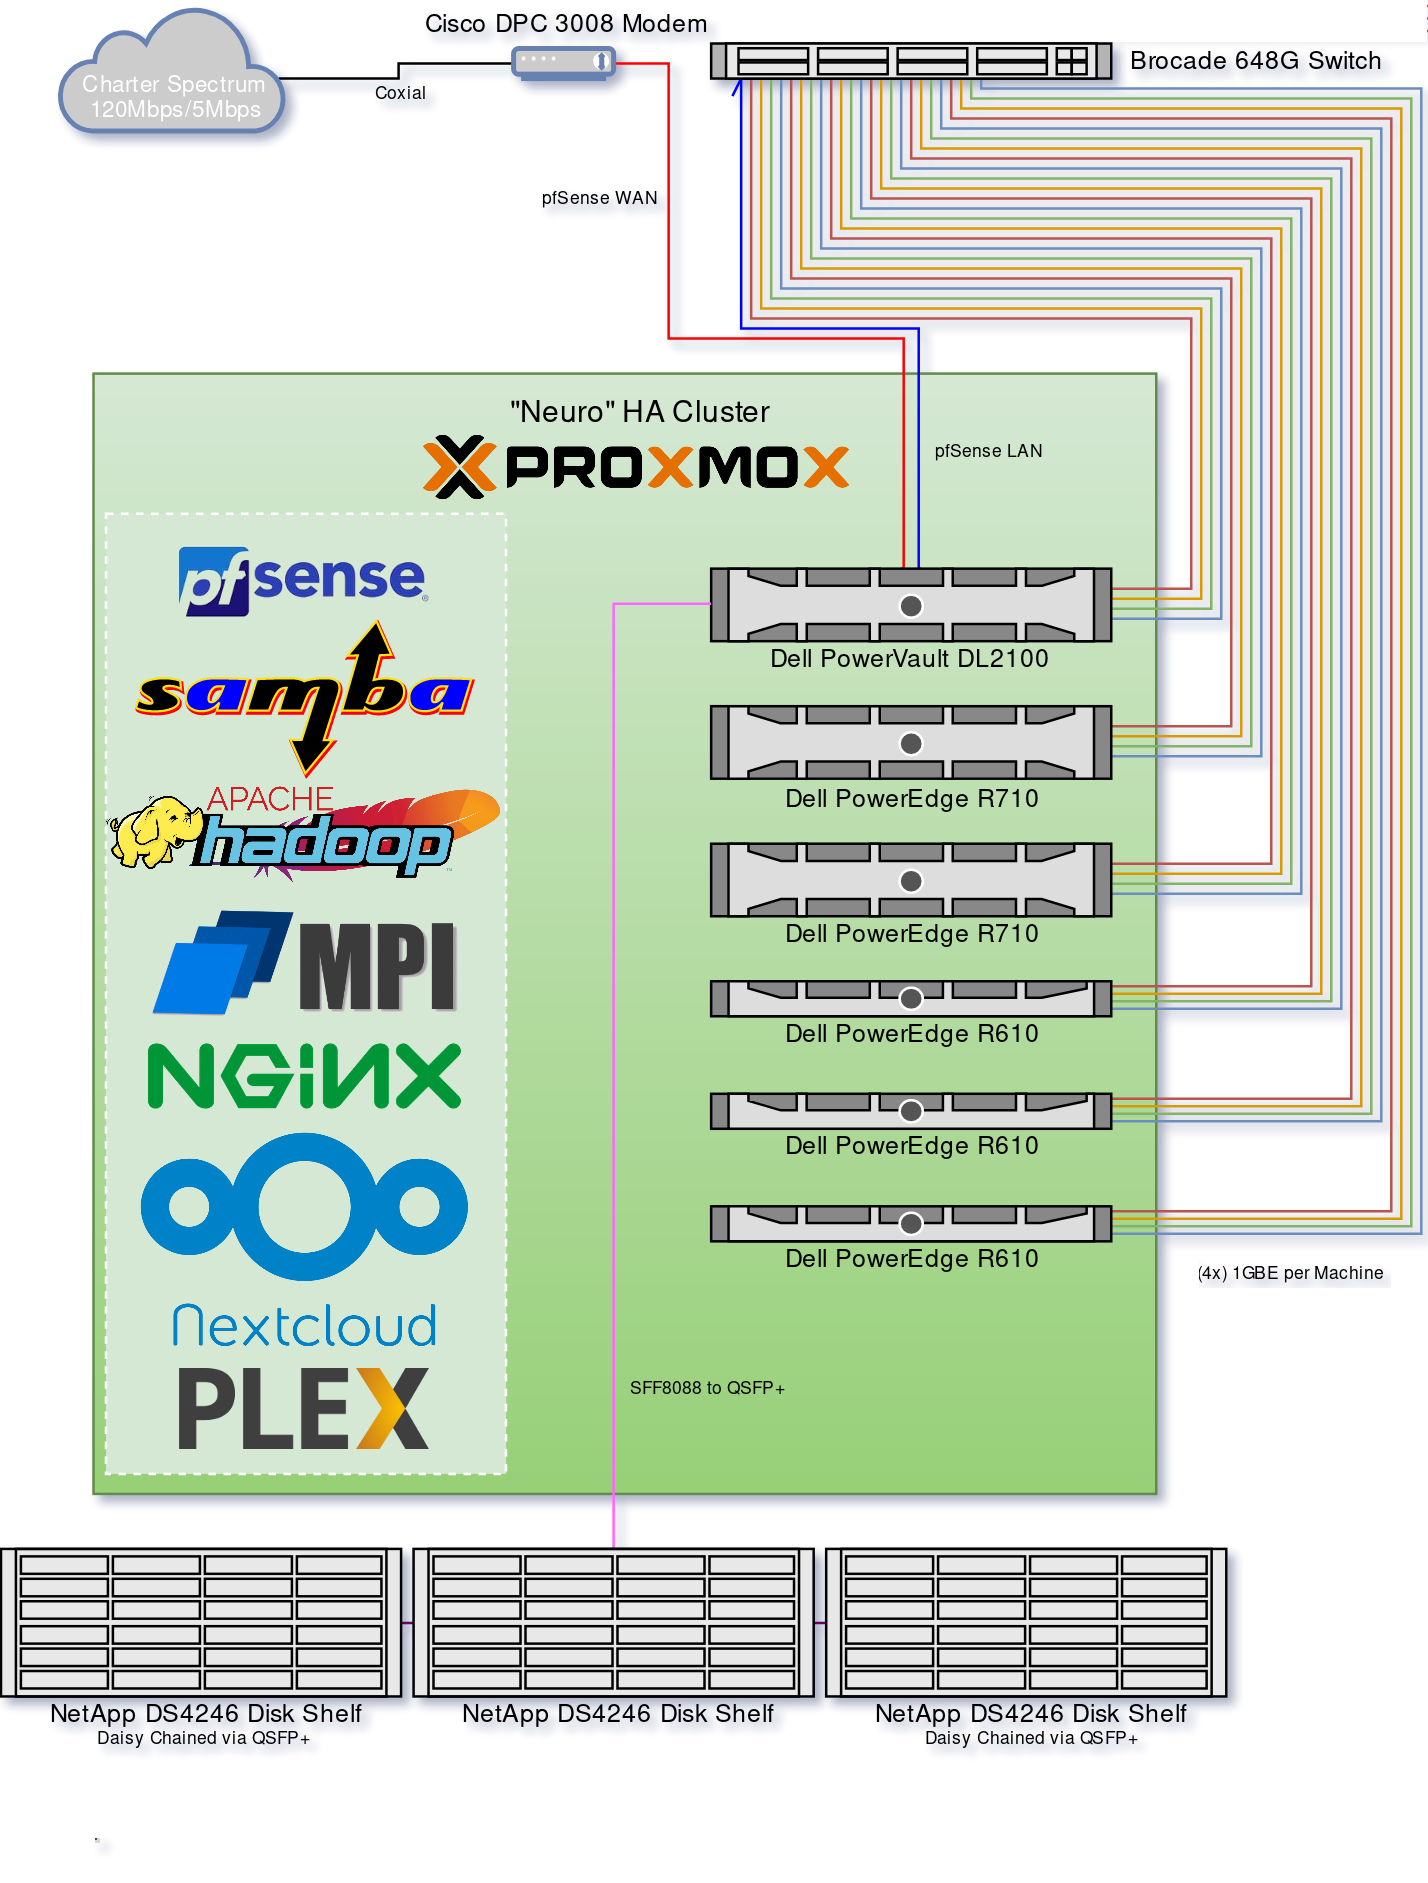
\includegraphics[width=7.9cm]{Images/Neuro_Network_Diagram_Small.png}
\caption{Neuro's Network Diagram}
\label{fig:Network Diagram}
\end{figure}

\begin{figure}[htp]
\centering
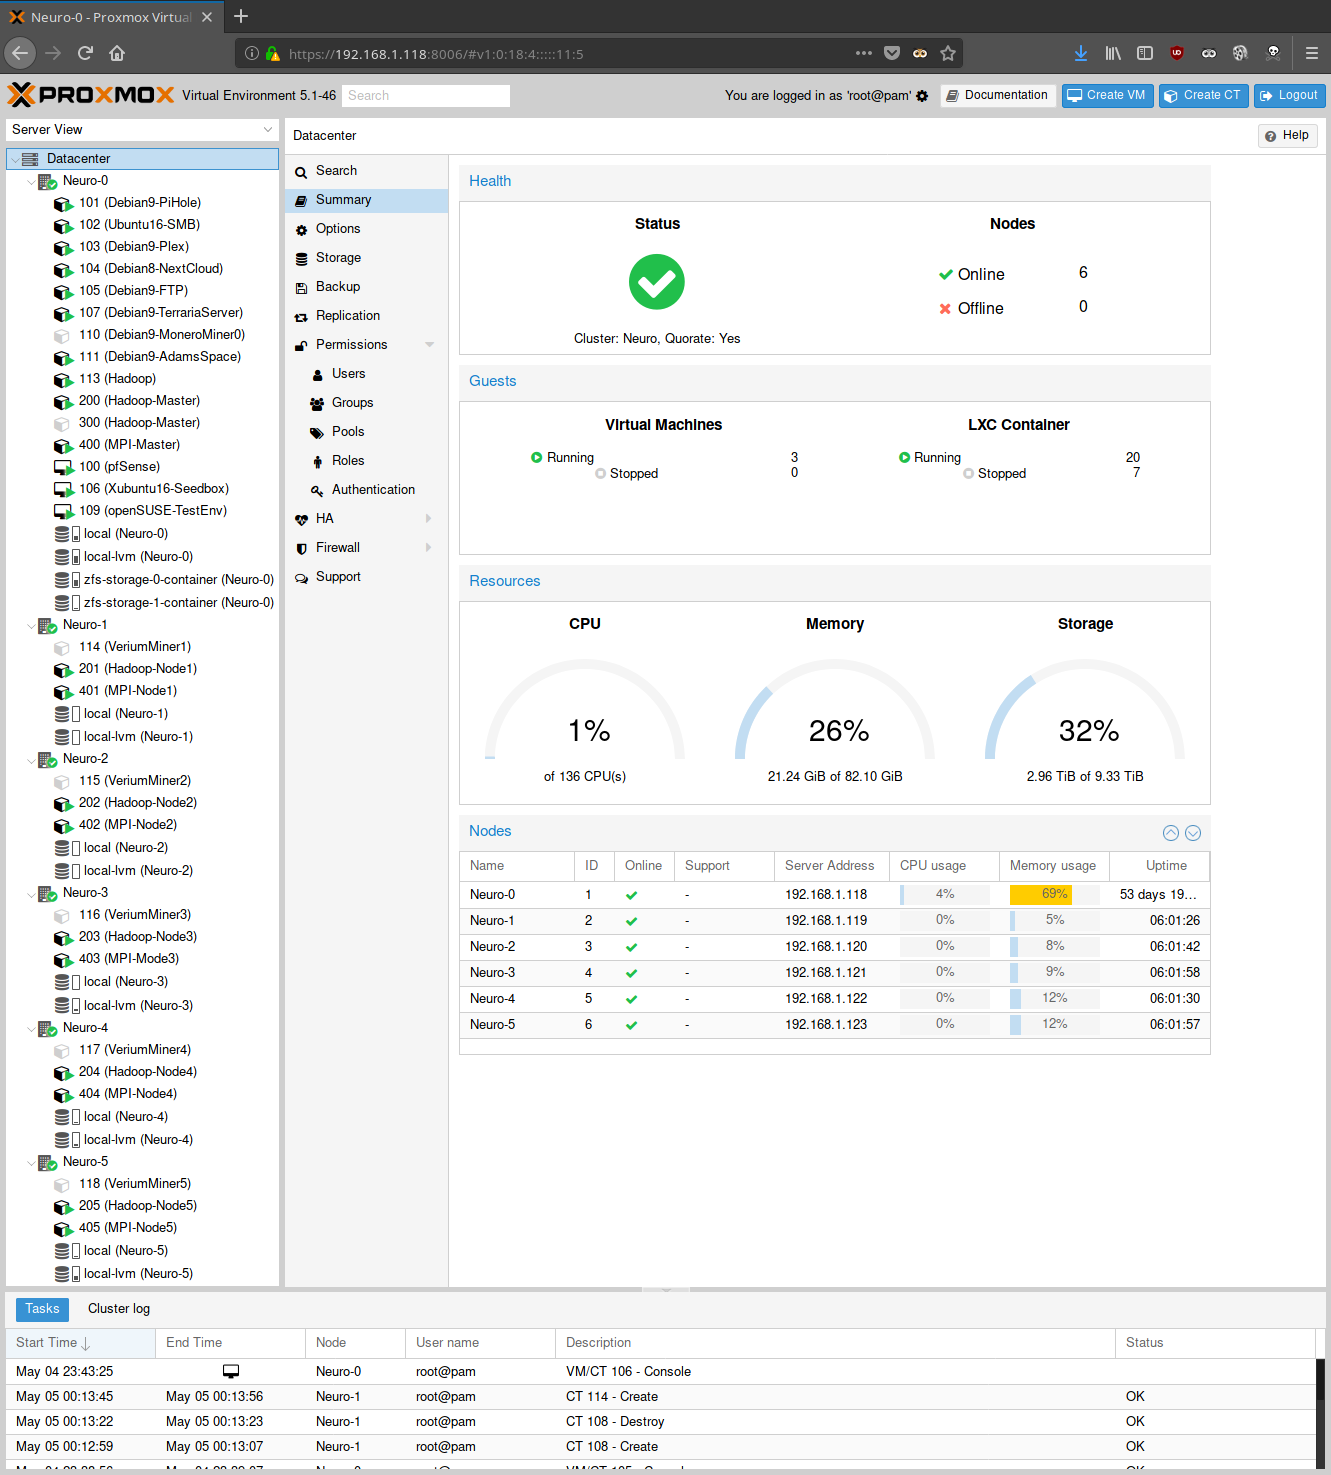
\includegraphics[width=7.9cm]{Images/proxmoxDashboard.png}
\caption{Proxmox Dashboard}
\label{fig:Network Diagram}
\end{figure}



\subsubsection{Apache Hadoop 3.1.0 \& Hadoop Yarn}
\indent For processing the dblp dataset, Apache Hadoop 3.1.0 was utilized configured in fully-distributed mode based on the Hadoop Apache wiki \cite{HadoopClusterWiki} using the openJDK 8 environment. It is configured in a six-node cluster with the master-node set as the primary namenode, the resource manager, and the secondary namenode. The other five worker nodes are set as the datanodes, resource manager, and namenodes as seen in figure 3 and figure 4 which shows the cluster architecture and the node architecture, respectively. \\
\indent The Hadoop Distributed File System (hdfs) is configured with a replication value of five for higher performance across all worker nodes as seen in figure 4, displaying the hdfs-site.xml configuration file. \\
\indent In the mapred-site.xml, shown in figure 5, the Mapper and Reducer workers are configured with a maximum allocation of 1024MB of memory for both Map and Reducer workers independently with the total allowed memory for all Map and Reducer workers together set to 4096MB. Gzip compression is set on the Mapper’s output to avoid memory overflow to swap. \\
\indent Shown in figure 6, on each worker node, the mapper and reducer functions are allocated with 4 vCores each with a maximum of 16 vCores allowed for both Map and Reducer workers. The container and resource manager vCores were not explicitly set so their default values were called. The Yarn scheduler is set with a maximum memory allocation of 6912MB and a minimum memory allocation of 128MB both with virtual memory checking disabled to ensure that containers are properly allocated on the openJDK 8 environment.  All map and reduce programs for Hadoop was written using the Python 2.7.3 scripting language executed using the Java Hadoop Streamer. 

\begin{figure}[htp]
\centering
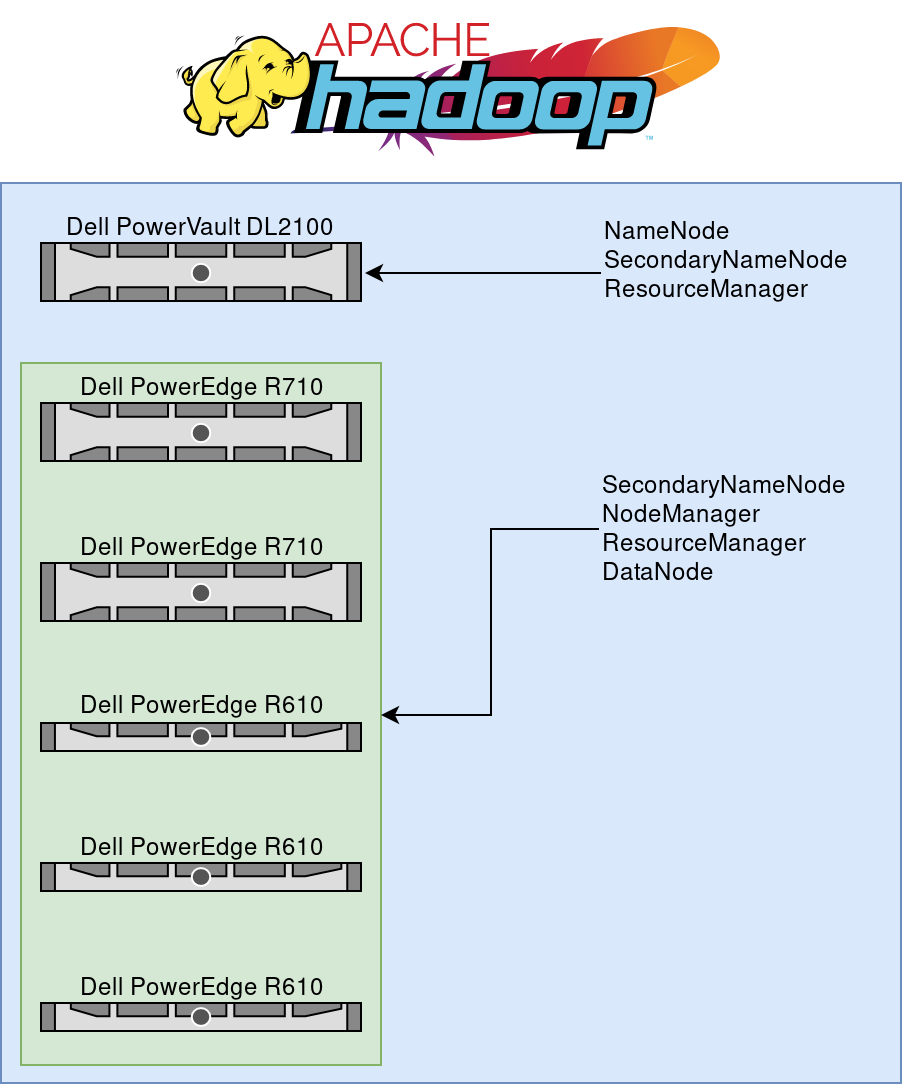
\includegraphics[width=7.9cm]{Images/Neuro_Hadoop_Architecture.png}
\caption{Hadoop Distributed Architecture}
\label{fig:Hadoop Architecture}
\end{figure}

\begin{figure}[htp]
\centering
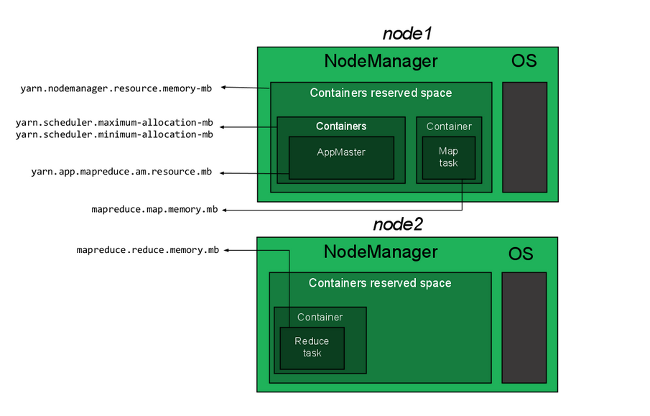
\includegraphics[width=7.9cm]{Images/hadoop-2-memory-allocation-new.png}
\caption{Hadoop Node Architecture}
\label{fig:Hadoop Architecture}
\end{figure}


\begin{minted}{xml}
<?xml version="1.0"?>
<?xml-stylesheet type="text/xsl" 
                 href="configuration.xsl"?>
<configuration>
  <property>
    <name>dfs.namenode.name.dir</name>
    <value>/home/hadoop/data/nameNode</value>
  </property>

  <property>
    <name>dfs.datanode.data.dir</name>
    <value>/home/hadoop/data/dataNode</value>
  </property>

  <property>
    <name>dfs.replication</name>
    <value>5</value>
  </property>
</configuration>
\end{minted}
\begin{figure}[htp]
\centering
\caption{Configuration for hdfs-site.xml}
\label{fig:}
\end{figure}

\begin{minted}{xml}
<?xml version="1.0"?>
<?xml-stylesheet type="text/xsl" 
                 href="configuration.xsl"?>

<configuration>
  <property>
    <name>mapreduce.framework.name</name>
    <value>yarn</value>
  </property>

  <property>
    <name>yarn.app.mapreduce.am.
            resource.memory-mb</name>
    <value>4096</value>
  </property>

  <property>
    <name>mapreduce.map.resource.
            memory-mb</name>
    <value>1024</value>
  </property>

  <property>
    <name>mapreduce.reduce.resource.
            memory-mb</name>
    <value>1024</value>
  </property>

  <property>
    <name>yarn.app.mapreduce.am.env</name>
    <value>HADOOP_MAPRED_HOME=
                /home/hadoop/hadoop</value>
  </property>
  <property>
    <name>mapreduce.map.env</name>
    <value>HADOOP_MAPRED_HOME=
                /home/hadoop/hadoop</value>
  </property>
  <property>
    <name>mapreduce.reduce.env</name>
    <value>HADOOP_MAPRED_HOME=
                /home/hadoop/hadoop</value>
  </property>
\end{minted}
\begin{figure}[htp]
\centering
\caption{Configuration for mapred-site.xml}
\label{fig:}
\end{figure}

\begin{minted}{xml}
<?xml version="1.0"?>
<configuration>

<!-- Site specific YARN 
                  configuration properties -->
  <property>
    <name>yarn.acl.enable</name>
    <value>0</value>
  </property>

  <property>
    <name>yarn.resourcemanager.hostname</name>
    <value>Hadoop-Master</value>
  </property>

  <property>
    <name>yarn.nodemanager.aux-services</name>
    <value>mapreduce_shuffle</value>
    </property>
<!-- vCore Allocation -->
  <property>
    <name>yarn.scheduler.
            maximum-allocation-vcores</name>
    <value>16</value>
  </property>
  <property>
    <name>yarn.scheduler.
            minimum-allocation-vcores</name>
    <value>4</value>
  </property>
  <property>
    <name>mapreduce.map.cpu.vcores</name>
    <value>4</value>
  </property>
  <property>
    <name>mapreduce.reduce.cpu.vcores</name>
    <value>4</value>
  </property>
<!-- Memory Allocation -->
  <property>
    <name>yarn.nodemanager.resource.
                            memory-mb</name>
    <value>6912</value>
  </property>

  <property>
    <name>yarn.scheduler.
                maximum-allocation-mb</name>
    <value>6912</value>
  </property>

  <property>
    <name>yarn.scheduler.
                minimum-allocation-mb</name>
    <value>128</value>
  </property>

  <property>
    <name>yarn.nodemanager.
                   vmem-check-enabled</name>
    <value>false</value>
  </property>
</configuration>
\end{minted}
\begin{figure}[htp]
\centering
\caption{Configuration for yarn-site.xml}
\label{fig:}
\end{figure}


\subsubsection{MPICHv2}
\indent For data aggregation and graphing, the message passing interface (MPI) version 3.2.1 was utilized to efficiently parallelize all the data. \\
\indent The MPI program is ran on all six of the same nodes as the Hadoop cluster although in separate LXC virtual containers with full physical resource allocation. The master node, node-0, only sends data and jobs to the rest of the nodes, nodes 1-5, which does all the computations. The reason why the master node does not do any computation is because the master nodes is already running about thirteen other virtual machines and containers running different services for other projects and personal use where as the nodes 1-5 are reserved strictly for computation. \\
\indent All the programs are built using the mpi4py library for the Python 2.7.3 scripting language.

\subsection{Data Set}
The data-set provided by dblp contained the essential meta-data required for the success of \textit{Collaboration Analysis}. The data-set contains characteristics such as the author, abstract, date published, and references. Along with the previous characteristics, each publication has a unique identifier tag, id, to avoid any form of collision or discrepancy in the process of digitally storing the publication. An example of the format of the id characteristic is: ``5626736c-e434-4e2d-8405-54940fab88ab``. The dblp data-set contains the meta-data for over four million publications by over two million authors and and spans over five thousand conferences. The data-base is about 2958MB in size. An example except of the data set is shown in figure 8.

\begin{figure}[htp]
\centering
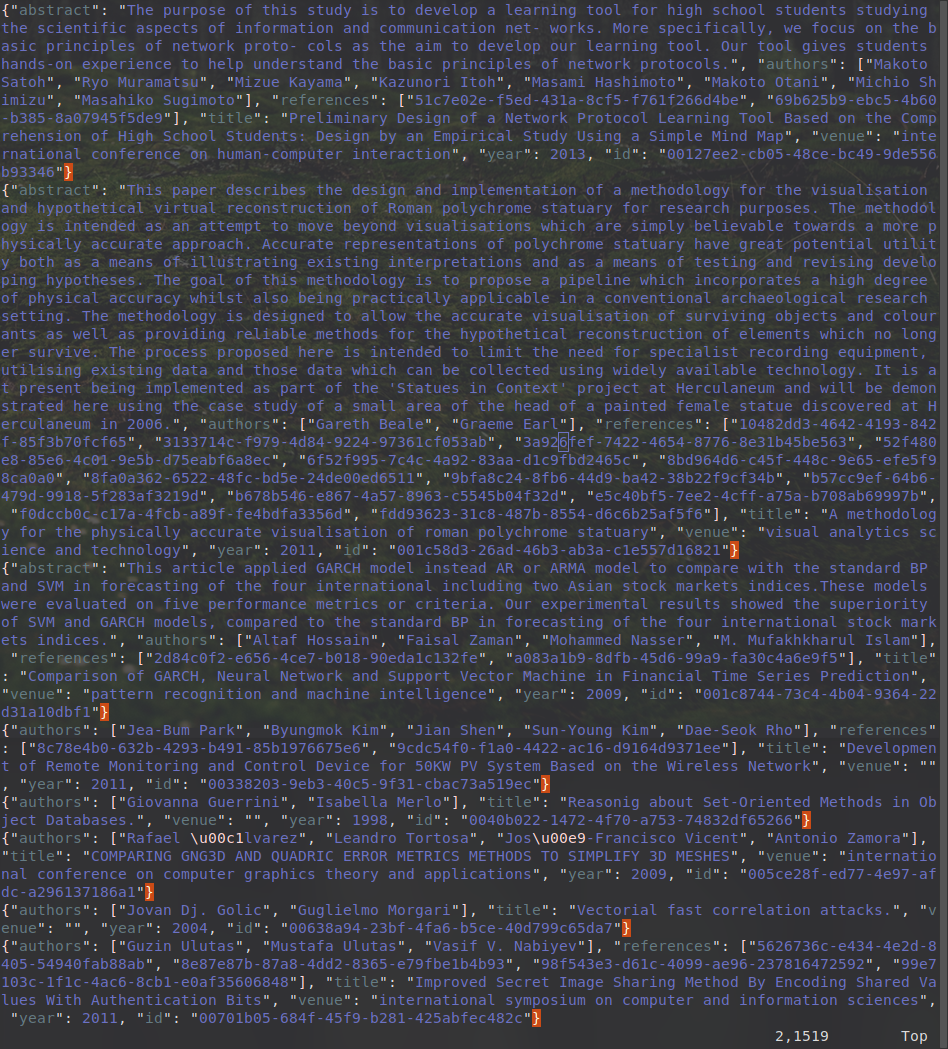
\includegraphics[width=7.9cm]{Images/dblp-data.png}
\caption{dblp Data Set}
\label{fig:}
\end{figure}


\subsection{MapReduce Programs}
\indent To collect and organize all the data from the dblp dataset, four sets of mappers and reducers were required. The four sets grabs the article ID and year published, grabs the authors and the article ID, grabs the ID and amount of times cited, and the last set counts the number of collaborations between different authors.
\subsubsection{Article-Year}
\indent The first set of programs grabs the year a publication was published along with the unique ID number. In order to do this the JSON file, provided by dblp, is converted into a regular expression as shown in figures 5 and 6. The mapper then searches for the term "id" followed by a colon and space. After finding the tag the program then searches for any combination of dashes, numbers, and lower case letters. After finding all IDs, the mapper then searches for the term "year" followed by a colon and a space. Within the year tag, any combination of numbers is found. The mapper program then send the mapper the data in the format of "ID(tab)year".\\
\indent In figure 6, the reducer operated by splitting the mappers output on the tab making the left-sided term the ID and the right-sided term the year. After splitting the mappers output, the reducer outputs to a text file in the format of "ID,year".

\begin{minted}{python}
#!/usr/bin/python
import sys,re
for line in sys.stdin:
  try:
    idNum = re.search(r'"id": 
        \"([0-9a-z\-]*)\"',line).group(1)
    year = re.search(r'"year": ([0-9]*)',
                           line).group(1)
    print '{0}\t{1}'.format(idNum,year)
  except AttributeError:
  continue
\end{minted}
\begin{figure}[htp]
\centering
\caption{Code for articleYearMapper.py}
\label{fig: articleYearMapper.py}
\end{figure}

\begin{minted}{python}
#!/usr/bin/python
import sys

for line in sys.stdin:
    idNum,year = line.split('\t')
    print '{0},{1}'.format(idNum,year)
\end{minted}
\begin{figure}[htp]
\centering
\caption{Code for articleYearReducer.py}
\label{fig: articleYearReducer.py}
\end{figure}

\subsubsection{Authors-Article}
The Author-Article set of mappers and reducers finds all publications and author has published.\\
\indent Figure 9 shows the code for the mapper. After converting the JSON file to a regular expression, the mapper searches for "id" followed by a colon and a space. After finding the identification tag, the mapper then accepts all combinations of strings exclusive to '[' and ']' characters. Then the mapper will looks for the tag "authors" followed by a colon and space. Upon finding the author identification tag, the mapper accepts all strings exclusive to '[' and ']' characters. Since the authors section of the JSON file is a list of authors separated by commas, the mapper will then split the list by the comma to only grab the names. Because of formatting issues with the JSON file itself a workaround had to be made for the reducer. The workaround takes all authors and replaces the quotation marks around their names and replaces them with a blank space. The mapper will also replace new lines in both the author and IDs with blank spaces before sending the data to the reducer in the format of "author(tab)ID".\\
\indent Figure 10 is the reducer for the authorArticles. The reducer is simple separating the output of the mapper on the tab character, taking the left-sided term as the author name and the right-sided term as the ID's. The reducer will then output to a file in the format of "author,ID".

\begin{minted}{python}
#!/usr/bin/env python
import sys,re

# Read each line from stdin
for article in sys.stdin:
  try:
    idNum = re.search(r'"id": \"([^\[|^\]]*)\"',
                               article).group(1)
    authors = re.search(r'authors":
             \[([^\[|^\]]*)\]',article).group(1)
    authors = authors.split(',')
    for author in authors:
      author = str(author).replace('"','')
      author = author.replace('\n','')
      idNum = idNum.replace('\n','')
      print '{0}\t{1}'.format(author,idNum)

  except AttributeError:
    continue
\end{minted}
\begin{figure}[htp]
\centering
\caption{Code for authorsArticlesMapper.py}
\label{fig: authorsArticlesMapper.py}
\end{figure}

\begin{minted}{python}
#!/usr/bin/env python
import sys

for line in sys.stdin:
    author, idNum = line.split('\t')
    author = author[1:]
    idNum.replace('\n','')
    print '{0},{1}'.format(author,idNum)

\end{minted}
\begin{figure}[htp]
\centering
\caption{Code for authorsArticlesReducer.py}
\label{fig: authorsArticlesReducer.py}
\end{figure}

\subsubsection{Citation Counter}
The citation counter Map Reducer program counts the number of citations that exists per article.\\
\indent Figure 12 shows the code for the citation counter. After converting the JSON file to a regular expression, the mapper will then find the string "references" followed by a colon and a space. After finding the references identification tag, the mapper will accept any combination of strings that include white spaces and characters, but are exclusive to asterisks, commas, and dashes. Upon parsing the references, the mapper will reformat the data to change any commas or new lines to blank spaces. After reformatting the data, the mapper will output in the format of "reference(tab)1".\\
\indent The reducer, shown in figure 13, will split the mapper output on the tab making the left-sided term the word and the right-sided term a simple '1'. After splitting the mapper output, the reducer will add the amount of ones a reference has and output to a text file in the format of "id,total".
\begin{minted}{python}
#!/usr/bin/env python
import sys,re

# Read each line from stdin
for article in sys.stdin:
  try:
    refs = re.search(r'references":
    \[([\w|\s|^"|^,|^-]*)\]',article).group(1)
    refs = refs.split(',')
      for ref in refs:
        ref = ref.replace('\n','')
        ref = ref.replace('"','')
        ref = ref.replace(' ','')
        print '{0}\t{1}'.format(ref, 1)
  except AttributeError:
  continue
\end{minted}
\begin{figure}[htp]
\centering
\caption{Code for citationCounterMapper.py}
\label{fig:}
\end{figure}

\begin{minted}{python}
#!/usr/bin/env python
import sys

curr_word = None
curr_count = 0

# Process each key-value
# pair from the mapper
for line in sys.stdin:
  # Get the key and value from the 
  # current line
  word, count = line.split('\t')
  # Convert the count to an int
  count = int(count)
  # If the current word is the same as the 
  # previous word, increment its count, 
  # otherwise print the words count to stdout
  if word == curr_word:
    curr_count += count
  else:
    # Write word and its number of occurrences 
    # as a key-value pair to stdout
      if curr_word:
        print '{0}\t{1}'.format(curr_word,
                                curr_count)
      curr_word = word
      curr_count = count

# Output the count for the last word
if curr_word == word:
  print '{0}\t{1}'.format(curr_word, 
                                 curr_count)

\end{minted}
\begin{figure}[htp]
\centering
\caption{Code for citationCounterReducer.py}
\label{fig:}
\end{figure}

\subsubsection{Collab Counter}
The set of mappers and reducers for collabCount counts the number of collaborations between different authors.\\
\indent After converting the JSON file to a regular expression, the mapper will look for the tag "authors" followed by a colon and white space and accepts strings of all characters. For formatting purposes, the mapper replaces all quotation marks with spaces and splits on the comma. The mapper will then output the in the format of "list of authors(tab)1".\\
\indent The reducer, shown in figure 15, will then find who collaborated with who and will output to a text file in the format of "Author name,amount of collaborative partners".

\begin{minted}{python}
#!/usr/bin/env python
import sys,re

# Read each line from stdin
for article in sys.stdin:
  try:
    authors = re.search(r'authors": 
        \[([^\[|^\]]*)\]',article).group(1)
    authors = authors.replace('"','')
    authors = authors.split(',')
    authors = ':'.join(authors)
    authors = '"' + authors + '"'
    print '{0}\t{1}'.format(authors, 1)
  except AttributeError:
    continue
\end{minted}
\begin{figure}[htp]
\centering
\caption{Code for collabCountMapper.py}
\label{fig:}
\end{figure}

\begin{minted}{python}
#!/usr/bin/env python
import sys

curr_word = None
curr_count = 0

# Process each key-value pair from the mapper
for line in sys.stdin:
  # Get the key and value from the 
  # current line
  word, count = line.split('\t')
  # Convert the count to an int
  count = int(count)
  # If the current word is the same as the 
  # previous word, increment its count, 
  # otherwise print the words count
  # to stdout
  if word == curr_word:
    curr_count += count
  else:
    # Write word and its number of occurrences
    # as a key-value pair to stdout
      if curr_word:
        print '{0}\t{1}'.format(curr_word, 
                                curr_count)

      curr_word = word
      curr_count = count

# Output the count for the last word
if curr_word == word:
  print '{0}\t{1}'.format(curr_word,
                                 curr_count)
\end{minted}
\begin{figure}[htp]
\centering
\caption{Code for collabCountReducer.py}
\label{fig:}
\end{figure}

\subsection{MPI Program}
The MPI program is built to parallelize all the data aggrecation. The program hashes all of the articles for easier searchability and merges the results from the MapReduce programs with the newly created hash. The output of the program is used to search and find the specific articles to analyze how many citations were made for the article which will allow the team to make conclusions on the article's success.   

The MPI program is built to paralellize all the data from the data aggregator. First, the program hashes all of the articles, for easier searchability, then merges the results from the MapReduce programs with the newly created hashes. Upon completion, the output of the program is used to search and find the specific article to analyze the amount of reference made to the article. This process will allow the team to make conclusions about how successful the publication  
\begin{minted}{python}
import mpi4py
mpi4py.rc.recv_mprobe = False
from mpi4py import MPI

def mergeDicts(x,y):
  commonKeys = list(set(x.keys())
                 .intersection(set(y.keys())))
    for key in commonKeys:
      x[key] = x[key] + y[key]
      del y[key]
  z = x.copy()
  z.update(y)

    return z


comm = MPI.COMM_WORLD
rank = comm.rank
size = comm.size

workers = range(1,size)
workList = [[] for x in range(size-1)]


if rank == 0:
  print 'Opening main file...'
  authArtFile = open('authorsArticlesFile2','r')
  masterDict = {}

  workerIndex = 0
  lineCounter = 0
  print 'Analyzing contents of file...'
  for line in authArtFile:
      if lineCounter == 2368495:
      print 'Allocating work for new worker ',
                                 workerIndex
      workerIndex += 1
      lineCounter = 0

      if workerIndex < size - 1:
        workList[workerIndex].
                  append(line.replace('\n',''))
      else:
        break

      lineCounter += 1

  print 'Closing main file...'
  authArtFile.close()

  print 'Sending work to workers...'
  for worker in workers:
    comm.send(workList[worker-1],dest=worker,tag=0)
    print 'Sent worker ',worker,' some data!'

  print 'Waiting for all workers to complete...'
  comm.Barrier()

  print 'Building master hash table...'
  for worker in workers:
    workerDict = comm.recv(source=worker,tag=1)
    masterDict = mergeDicts(masterDict,workerDict)

  print 'Saving to file...'
  authArtDictFile = 
            open('authorArticleDictFile','w')
  for author,idList in masterDict.items():
    fileLine = author + ':' + idList + '\n'
    authArtDictFile.write(fileLine)

  authArtDictFile.close()

  print 'Done!'


else:
  data = comm.recv(source=0,tag=0)
  print 'I am worker ',rank,
    ' and I received data of size ',len(data)

  workerDict = {}

  progressCounter = 0
  for entry in data:
    if progressCounter %  100000 == 0:
      print 'Worker ',rank,' is processing..'
      progressCounter = 0

    author,idNum = entry.split(',')
    if author not in workerDict.keys():
      workerDict[author] = [idNum]
    else:
       workerDict[author].append(idNum)
    progressCounter += 1

  print 'I am worker ',rank,
            ' and I am finished. Sending...'
  comm.ssend(workerDict,dest=0,tag=1)

\end{minted}
\begin{figure}[htp]
\centering
\caption{Code for hashTableGen.py}
\label{fig:}
\end{figure}

\section{Evaluation}
All three members have been working diligently on this project. Since the beginning of this project there have been at least three meetings per week dedicated to working on this project. Each meeting consisted of anything from brainstorming to writing code and tuning the Hadoop cluster. Despite our efforts, at the time of writing this paper, the cluster is still processing the data we have given it. When the results of the processing have been produced, the team plans to analyze the data with varying tools and statistical analysis. 

We hope to derive three features of data from our analysis: the number of collaborations between a given set of authors, the number of citations of a given collaboration, the standard deviation of the author's individual citations before a certain collaboration and the author's total average citations before and after a certain collaboration. Of these features, we are interested in seeing if there exists any sort of correlation between them. If there does exist a correlation, we hope to derive a rationale behind it's existence.

\section{Member Contribution}
\subsection{Adam Montano}
Adam Montano's role \cite{macro_malware}in the team was the project manager along with being one of the coders. Montano's primary role was to manage meeting times, due dates, and keep track of finished and managing which models were finished or unfinished. He focused on helping Gabriel learn Python and work together with Gabriel to design the regular expressions necessary for Hadoop MapReduce. Montano was also the primary coder for the portion of the project that required MPI, along with the primary analyst for the final analysis of the data. 

\subsection{Brandon Thai Nguyen}
Brandon Thai Nguyen's role in the team was the system architect and the development operator. Nguyen's primary role was to deploy the vitalization cluster and ready it for production. He focused on setting up Apache Hadoop 3.1.0 and tuning the parameters of the program for maximum throughput. Nguyen also built the testing environments and built automation scripts to load the hdfs, as well as read logs to debug the Hadoop cluster MPI cluster, MapReduce programs, and MPI programs.

\subsection{Gabriel Fukumoto}
Gabriel Fukumoto's role in the team was to assist Adam Montano in the coding process. Fukumoto's primary role was to help Adam figure out what modules would be considered necessary, assist with the creation of regular expressions to be parsed, and implement the algorithms created by Montano and Fukumoto. He focused on learning the nuances of MapReduce Python programming\cite{Python}. Fukumoto also assisted in debugging and algorithm creation during the implementation and beginning processes.

\section{Discussion}
Since this is the groups first exposure to both Big Data and Apache Hadoop, problems are expected. Although some were able to be solved, others were not. Because of this, certain portions of the project were able to be improved, while other portions had to be removed.

\subsection{Apache Hadoop 3.1.0}
Configuration of the pseudo-distributed Hadoop system was necessary to allow MapReduce programs to make process. Due to the Apache Hadoop 3.1.0 for pseudo-distributed systems wiki \cite{HadoopPseudoDistWiki}, the configuration was extremely straightforward and offered little to no resistance. However, due to lack of experience with Apache Hadoop and its resource manager, YARN, configuring a fully-distributed system brought up a myriad of problems.

\subsubsection{Heterogeneous Server Cluster}
The main problem with ``Neuro``, the server cluster, is that none of Neuro's node are identical. Because of this issue, parameter tuning became a problem as Hadoop was built to run on fully homogeneous clusters. To alleviate this issue, Neuro's resources were allocated according to the weakest node in the cluster in order. This fix was necessary to avoid improper allocation of Hadoop's container resources such as the amount of virtual cores allocated for map/reduce workers; or the improper setting of resource managers and memory allocation for the map/reduce block size. The latter primarily occurred on node that had less physical CPU cores or logical thread, along with nodes that had less memory.

\subsubsection{MrJob Python Library}
Yelp's MyJob was attempted to be utilized to keep the programming work-flow as efficient as possible. MrJob's benefits are that both the mapper and reducer workers are kept as separate functions in a single program file, multi-step MapReduce jobs are able to be created, the ability to test programs in a local machine environment before moving it to the full cluster, and the portability between different services such as: Apache Hadoop Spark, Amazon Elastic MapReduce, and Google Cloud DataProct.\\
\indent The installation of MrJob was easy since it utilized pip to install the library. Unfortunately, running any Python programs in MrJob resulted in the Java job streamer to fail. By looking at the Hadoop logs it was revealed that Hadoop YARN was having an issue reading input files, even though it was loaded into the hdfs. While the problem was never resolved, the team instead wrote normal Python MapReduce programs to alleviate the issue.

\subsection{MPICHv2}
The configuration of MPICHv2 was relatively straight forward. However, due to lack of experience, it was initially configured to run on one core or MPI slot per node. This was quickly alleviated by creating a hosts configuration file defining how many slots to allocate per node.

\subsection{Opportunities of Potential Collaboration}
One of the modules that had to be removed due to time constraints was finding the opportunity of potential collaborations between authors. The method planned to be used was brought up by Adam Montano as he is currently enrolled in a class for social networks. The plan was to find authors whom had a mutual collaborative partner and calculate if the collaboration was viable based upon how many nodes separated them and how relevant the topics they wrote about were towards each other. This module would have utilized the abstract of the publications which were included in the JSON files provided to the team by dblp. 

\subsubsection{Stretch goal}
Although the above mentioned was going to be the primary way the team calculated potential opportunities for collaboration, the team also had another idea building upon the previously mentioned. The problem with the aforementioned idea was that another identification tag in the JSON file was the publisher of the paper. This led to be a problem because the influence of the publisher could mean that authors could only collaborate with researchers who generally published with the same publisher. To get around this, the group came up with the idea to match people edge-to-edge globally rather than just edge-to-edge based upon the same parent node. The idea is to match everyone with everyone to see if it was viable or not rather than basing it upon an authors close social network. But, due to time constraints and unknowing of Neuro's processing ability the team had to remove this module.

\subsection{MapReduce Programming}
Programming the MapReduce programs had some strange quirks to it. All the programs had to ignore attribute errors when parsing through the dblp dataset. Another strange quirk about creating the MapReduce programs was that for certain tags, the reducer required the mapper to reformat the way the data was output. The mapper required the removal of commas, new lines, and quotation marks with white space and new lines being put in their place being put in their place. This made no sense as theoretically a JSON file is supposed to be formatted uniformly.

\subsection{MPI Programming}
The primary difficulty of MPI programming was trying to understand how the call blocking functions like comm.send and comm.recv which send and receives messages, respectively. To solve the problems, orders of worker operations had to be heavily evaluated to ensure that no call blocking functions would block the work of itself and other workers.

\section{Conclusion}
Through \textit{Collaboration Analysis} the team learned the architecture of Apache Hadoop and MPI architecture along with MapReduce and MPI programming by doing this project. The \textit{Collaboration Analysis} taught the team how to approach Big Data problems algorithmically and pragmatically. \textit{Collaboration Analysis} strides to find a correlation between an author, their publication, and their collaborative partners to justify whether or not the said publication may be considered a successful publication.


% if have a single appendix:
%\appendix[Proof of the Zonklar Equations]
% or
%\appendix  % for no appendix heading
% do not use \section anymore after \appendix, only \section*
% is possibly needed

% use appendices with more than one appendix
% then use \section to start each appendix
% you must declare a \section before using any
% \subsection or using \label (\appendices by itself
% starts a section numbered zero.)
%


% use section* for acknowledgment
\ifCLASSOPTIONcompsoc
  % The Computer Society usually uses the plural form
  \section*{Acknowledgments}
\else
  % regular IEEE prefers the singular form
  \section*{Acknowledgment}
\fi


The authors would like to thank the University of Nevada, Reno and the professor of CS 491.691.1004, Big Data, Feng Yan for giving them the opportunity to not only work on this project but give them their first real-world experience of using Apache Hadoop, Message Passing Interface, and what Big Data really is like.


% Can use something like this to put references on a page
% by themselves when using endfloat and the captionsoff option.
\ifCLASSOPTIONcaptionsoff
  \newpage
\fi



% trigger a \newpage just before the given reference
% number - used to balance the columns on the last page
% adjust value as needed - may need to be readjusted if
% the document is modified later
%\IEEEtriggeratref{8}
% The "triggered" command can be changed if desired:
%\IEEEtriggercmd{\enlargethispage{-5in}}

% references section

% can use a bibliography generated by BibTeX as a .bbl file
% BibTeX documentation can be easily obtained at:
% http://mirror.ctan.org/biblio/bibtex/contrib/doc/
% The IEEEtran BibTeX style support page is at:
% http://www.michaelshell.org/tex/ieeetran/bibtex/
%\bibliographystyle{IEEEtran}
% argument is your BibTeX string definitions and bibliography database(s)
%\bibliography{IEEEabrv,../bib/paper}
%
% <OR> manually copy in the resultant .bbl file
% set second argument of \begin to the number of references
% (used to reserve space for the reference number labels box)

\bibliography{citations}
\bibliographystyle{unsrt}
% You can push biographies down or up by placing
% a \vfill before or after them. The appropriate
% use of \vfill depends on what kind of text is
% on the last page and whether or not the columns
% are being equalized.

%\vfill

% Can be used to pull up biographies so that the bottom of the last one
% is flush with the other column.
%\enlargethispage{-5in}



% that's all folks
\end{document}


